

\chapter{DATA ANALYIS}

\section{Source of the Data }
\label{source-of-the-data}


To study the relationship between the SNP rs1059703 mutant haplotype and
its combined effects along with IRAK-1A/ IRAK-1C heterozygous splice
variants, data from NCBI's SRA database containing RNA-seq data of human
peripheral blood mononuclear cells from 15 patients were taken. This
study was conducted by Columbia University in 2016, with the Bio project
ID PRJNA343985 and the Geodata set accession number GSE87290 {[}261{]}.\cite{1}

Based on data from previous studies, the contributors Fergueson and Xue,
{[}{]} selected only the individuals in the top (high-responders) and
bottom (low-responders) extremes for inflammatory responses from
previous studies. These patients were subjected to inpatient endotoxin
challenge (1ng/kg LPS) in healthy humans. RNA-Seq was conducted for
peripheral blood mononuclear cells (PBMC, n=15) before and after LPS
administration. As previously stated, human monocyte cells predominantly
expressed IRAK-1A, with minimum levels of IRAK-1C expression. This
allowed the sensitive recording of changes in IRAK-1C mRNA levels
{[}261{]} (Refer Appendix A.).

\section{ Data processing.}\label{data-processing.}

The experimental SRA runs from NCBI were aligned with the identifier
sequences in table 5.2 using SRA Blast. The total number of perfect
matches was counted. These values were later normalized by dividing them
by the number of Giga{}{{}base pairs (Gbp) of each SRA read's data file to
give a normalized value. This data was processed using Python, R, and
Jupyter Notebooks for statistical calculations.

\textbf{Table 5.1} SRA Blast Query Sequences. Key sequences bolded and underlined.
%
% \begin{table}[]
% \textbf{Query Identifier} & \textbf{Query sequence}\tabularnewline
% \midrule
% IRAK-1A WT & \emph{CCCA}GGTGTACGAGAGGCTAGAGAAGCTGCAGGCAGTGGTG
%
% GCGGGGGTGCCCGGGCATT\textbf{T}\tabularnewline
% IRAK-1A Var & \emph{CCCA}GGTGTACGAGAGGCTAGAGAAGCTGCAGGCAGTGGTG
%
% GCGGGGGTGCCCGGGCATT\textbf{C}\tabularnewline
% IRAK-1C WT & \emph{ATCT}GGTGTACGAGAGGCTAGAGAAGCTGCAGGCAGTGGTG
%
% GCGGGGGTGCCCGGGCATT\textbf{T}\tabularnewline
% IRAK-1C Var & \emph{ATCT}GGTGTACGAGAGGCTAGAGAAGCTGCAGGCAGTGGTG
%
% GCGGGGGTGCCCGGGCATT\textbf{C}\tabularnewline
% \bottomrule
% \end{table}

\section{Statistical processing \&
analysis}\label{statistical-processing-analysis}

All statistical analysis were performed in Jupyter notebooks using
python. The Shapiro test for normalcy to determine the normalcy of the
variables under study~and secondly subjectively by observing the
histograms and box plot outputs {[}262{]}. To determine if there were
significant differences between two groups of paired data, a paired-T
test was performed for parametric data {[}266{]} and a Wilkson-paired
T-test {[}264{]} for non-parametric data based on the Shapiro-test
results. Independent and non-parametric groups were compared using the
Whitney-Mann U test and the Kruskal-Wallis test for significant
differences{[}265, 266{]}.

\begin{enumerate}
\def\labelenumi{\arabic{enumi}.}
\item
\end{enumerate}

\chapter{RESULTS}


\section{ Data Demographics}\label{data-demographics}

% \textbf{Table 6.1}
%
% \begin{longtable}[]{@{}llll@{}}
% \toprule
% & \textbf{Males (n)} & \textbf{Females (n)} &
% \textbf{Total}\tabularnewline
% \midrule
% \endhead
% \textbf{Total Participants} & 8 & 7 & 15\tabularnewline
% & & &\tabularnewline
% \textbf{Ethnicity} & & &\tabularnewline
% Caucasian & 6 & 3 & 9\tabularnewline
% African American & 2 & 4 & 6\tabularnewline
% & & &\tabularnewline
% \textbf{Inflammation response:} & & &\tabularnewline
% High & 4 & 4 & 8\tabularnewline
% Low & 4 & 3 & 7\tabularnewline
% & & &\tabularnewline
% \textbf{By Genotypes:} & & &\tabularnewline
% & & &\tabularnewline
% \emph{Homozygotes} & & & 7\tabularnewline
% IRAK-1A(WT) Homozygote & 5 & 0 & 5\tabularnewline
% IRAK-1A(Var) Homozygote & 3 & 0 & 2\tabularnewline
% & & &\tabularnewline
% \emph{Total Heterozygotes} & \textbf{-} & 7 & 8\tabularnewline
% IRAK-1A(WT) / IRAK-1A(Var) & \textbf{-} & 4 & 4\tabularnewline
% IRAK-1A(WT) / IRAK-1C(WT) & \textbf{-} & 2 & 2\tabularnewline
% IRAK-1A(Var) / IRAK-1C(VAR) & \textbf{-} & 1 & 2\tabularnewline
% \bottomrule
% \end{longtable}

\section{ Exposure to LPS causes a reduction of IRAK-1 mRNA
expression}\label{exposure-to-lps-causes-a-reduction-of-irak-1-mrna-expression}


While the roles of cytokines in inflammation have been extensively
studied, the genetics of their regulatory molecules have not from the
transcriptomic point of view. Recent studies on inflammatory responses
have shown that differential gene expression can lead to changes in the
inflammatory response, primarily through variances in mRNA levels. To
detect changes in the mRNA levels, the total IRAK-1 mRNA expressions per
Gbp before (median=2.7) and after the LPS (median=1.8) treatment were
compared. We tested for normalcy using the Shapiro-Wilk test, which
showed that the data was not normally distributed. Hence, we conducted
non-parametric tests were conducted. The Wilcoxon paired test indicated
that there was a significant difference between the median of the two
groups. Fig. 6.1B a drop of 0.78 mRNA counts per Gbp (p-value:0. 0.005)
(Fig. 6.1A).

To understandthe rate of change in IRAK-1 levels, linear regression
analysis was performed with the IRAK-1 levels before LPS treatment
against the expression levels after LPS administration. The linear model
had an R2 value of 0.31 and a slope of 0.74, with an intercept of
-0.249. This data suggests that the changes in IRAK-1 levels following
LPS treatment are significant but are primarily dependent on IRAK-1's
initial levels.


%\includegraphics[width=9.79292in,height=3.34615in]{media/image1.jpeg}

\textbf{Figure 6.1} TLR4 mediates the recognition of the antigen LP and
is responsible for the initiating-anti-microbial inflammatory response

\section{IRAK-1C levels remain constant as they fail to disengage from
the adaptor proteins
}\label{irak-1c-levels-remain-constant-as-they-fail-to-disengage-from-the-adaptor-proteins}

IRAK-1 has tw

%\includegraphics[width=9.83044in,height=5.32051in]{media/image2.png}\textbf{Figure 6.2} TLR4 mediates the recognition of the antigen LP and is responsible
%for initiates anti-microbial inflammatory response

\section{The role of IRAK-1 in Hyperinflammation
}\label{the-role-of-irak-1-in-hyperinflammation}

There have been a variety of studies that have sought to understand the
dynamics of the TLR-NF-kB pathway in inflammation, as an attempt to
develop possible therapies aimed at restoring cytokine regulation in
sepsis. These studies often implicate IRAK-1 as a key mediator in
regulating the intensity of endotoxin challenges. High levels of IRAK-1
expression has been associated with increased proinflammatory activity,
whereas Studies on LPS-tolerance in human monocytes revealed unaltered
TLR4 expression but suppressed MyD88-TLR4 and IRAK1-MyD88 interactions,
IRAK1 activation. As we had shown in section 6.1,IRAK-1 activation is
which is marked by a sharp decrease in IRAK-1 expression. Based on
previous studies, and our results from section 6.3, this drop is
primarily due to the phosphorylation of IRAK-1A splice variant.

In order to understand the impact of splice variants on the inflammatory
responses, it is essential to study the dynamics of IRAK-1 expression
levels amongst patients with high and low endotoxin sensitivities.
Figure 6.3 shows the levels of IRAK-1 and its splice variants amongst
patients with high and low sensitivity to endotoxin challenges before
and after LPS administration. Based on the results of the Shapiro-Wilk
test, we conducted both parametric and non-parametric tests to compare
IRAK-1A, IRAK-1C and the total IRAK-1 Levels before and after the LPS
treatments.

Table 6.2 summarizes the descriptive statistics of the groups under
study. We report a significant change in total IRAK-1 levels between
patients with low (p=0.03), and the high levels of inflammation
(p=0.0053). Similar to our results in 6.3, we obtained s significant
change in IRAK-1A levels as well low (p=0.013), and the high levels of
inflammation (p=0.010). Similar to our previous results, IRAK-1C failed
show exert any significant difference with. A p-value of 0.86 for
patients with high IRAK-1

% 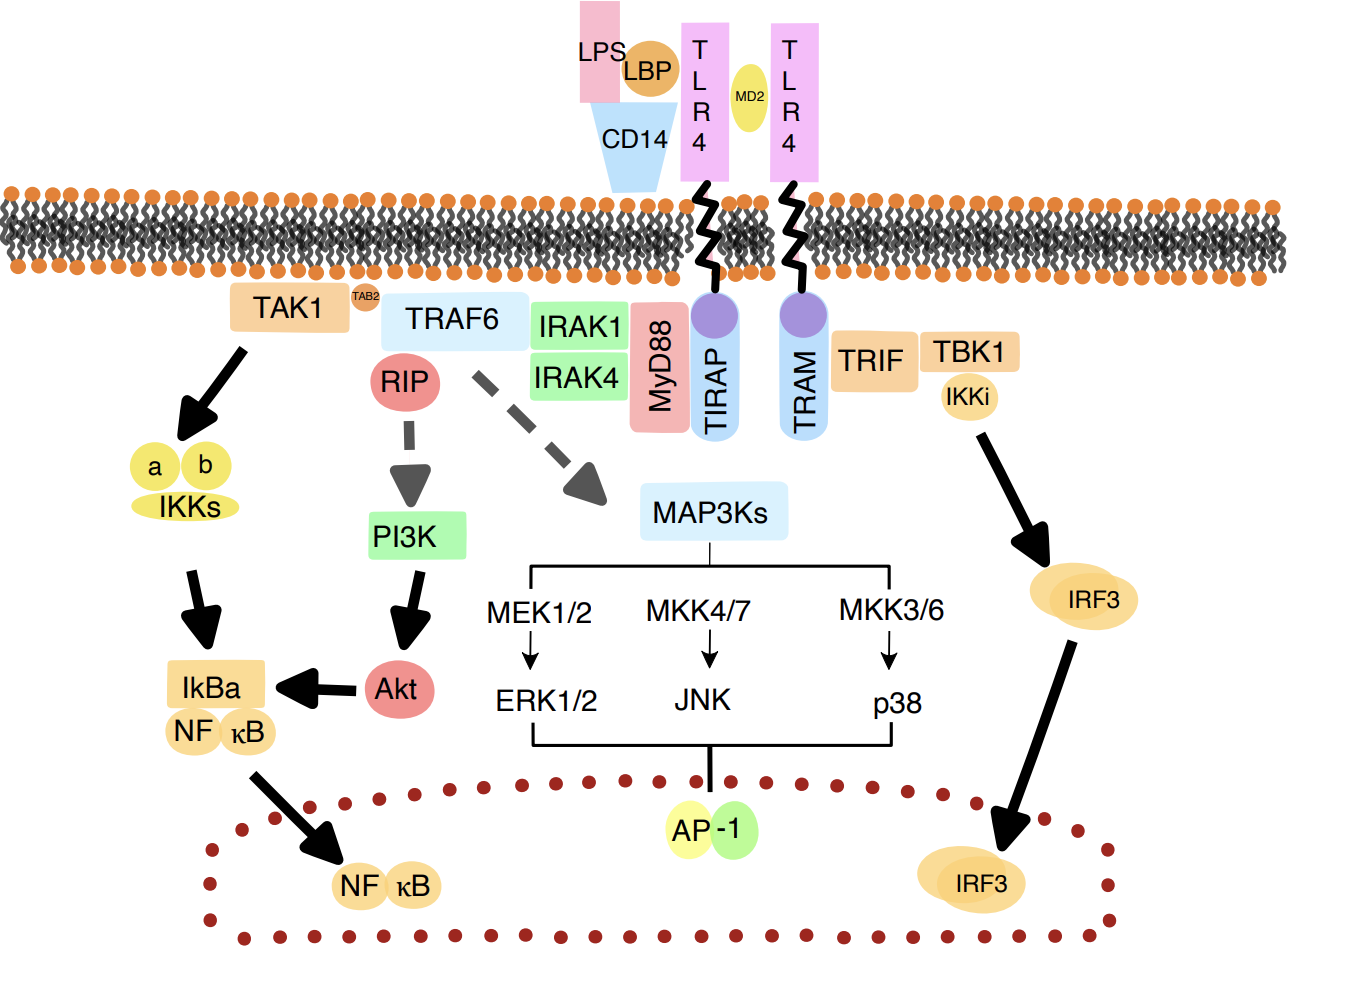
\includegraphics[width=9.38854in,height=6.39437in]{/thesismd/Aspose.Words.d7b25155-4470-43de-b824-aa5acef2e9e8.003.png}
%
%\textbf{Figure 6.3} TLR4 mediates the recognition of the antigen LP and
%is responsible for initiates anti-microbial inflammatory response
